
Le problème est que le résultat est satisfaisant visuellement, mais après exploitation (expliquée ci-dessous) on s'est rendu compte que l'on avait pas des résultats très cohérent suivant si on se trouvait dans un champs proche ou lointain. par exemple une distance entre têtes dans un champs lointain parraissait cohérente tandis que une distance entre têtes dans un champs proche était beaucoup trop grande. On a donc décidé de corriger cette carte de profondeur en lui appliquant une transformation.

Pour se faire, et comme c'est les têtes qui nous intéressent, on s'est appuyé sur elles pour corriger la carte de profondeurs. En effet, avec un peut de recherche dans la litérature on comprend que les têtes font sensiblement toutes la même taille, en tout cas qu'il y a une faible variance dans la population.

Et justement grâce à notre modèle finetuné de \textit{Yolov11}, pour les têtes detectés on a une boite englobante de la tête qui est assez précise. Par ailleur,  on a la relation suivante 

\begin{figure}
    \centering
    % \includegraphics[width=0.8\textwidth]{depth_correction_formula.png}
    \caption{Schémas de l'optique d'un appareil photo.}
    \label{fig:depth_correction_formula}
\end{figure}

\begin{equation} \label{eq:camera_relation}
    \frac{\text{width (pxl)}}{\text{focale (pxl)}} = \frac{\text{width (m)}}{\text{depth (m)}}
\end{equation}


comme notre focale d'appareil est une constante, alors le produit $ \text{width} \times \text{depth} $  est proportionnel à la taille de la tête et doit donc être également répartie et ne pas dépendre de la prodonfeur, hors ce n'est pas ce que l'on observe, on voit nettement une correlation. 

\begin{figure}
    \centering
    % 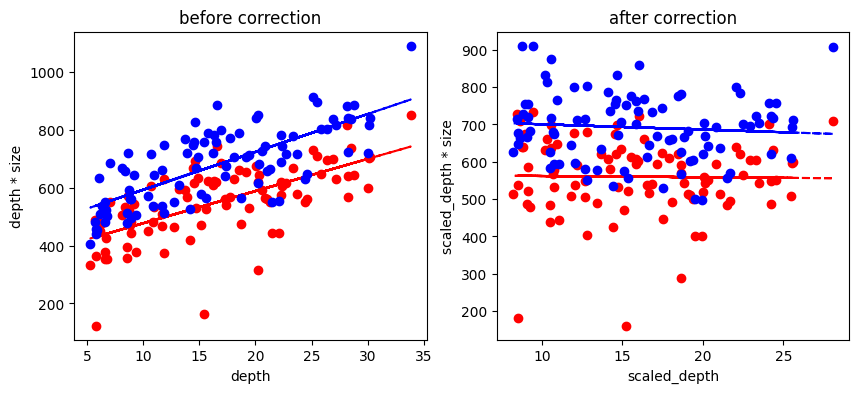
\includegraphics[width=0.8\textwidth]{depth_correction.png}
    \caption{(à gauche) avant la correction, on voit la corrélation. (à droite) la correction annule la correlation. }
    \label{fig:depth_correction}
\end{figure}

On effectue donc une régression linéaire pour déterminer une correctione linéaire à la carte de profondeur qui permet d'annuler la correlation entre le produit expliqué et la taille des têtes.

